\documentclass[a4paper,10pt]{article}

\usepackage[hidelinks]{hyperref}
\renewcommand{\figureautorefname}{Figura}
\renewcommand{\subsectionautorefname}{Sottosezione}
\usepackage{float}
\usepackage{tabularx}

% Lingua 
\usepackage[utf8]{inputenc}
\usepackage[T1]{fontenc}
\usepackage{lmodern}
\usepackage[italian]{babel}

% Margini
\usepackage{geometry}
\geometry{a4paper, top=3cm, bottom=3cm, left=3cm, right=3cm}
\setlength{\parindent}{0pt}

\usepackage{graphicx}   % per immagini
\usepackage{caption}    % per didascalie
\captionsetup[table]{labelformat=empty}
\usepackage{ifthen}     % per \ifthenelse
\usepackage{longtable}

\usepackage{array}      % per tabelle
\newcolumntype{M}[1]{>{\centering\arraybackslash}m{#1}}

\usepackage{datetime}

% Definisci un formato personalizzato
\newdateformat{italianformat}{\THEDAY~\monthname[\THEMONTH]~\THEYEAR}
\newdate{dataverbale}{04}{04}{2026}

% Definizione del formato con le barre
\newdateformat{slashdate}{\twodigit{\THEDAY}/\twodigit{\THEMONTH}/\THEYEAR}

% Per logo in ogni pagina
\usepackage{eso-pic}
\usepackage{tikz}
\AddToShipoutPictureBG{%
  \ifthenelse{\value{page}>1}{%
    \begin{tikzpicture}[remember picture, overlay]
      % Icona
      \node[anchor=north west, inner sep=0pt] at ([xshift=28pt,yshift=-28pt]current page.north west) 
        {
\includegraphics[width=1cm, height=1cm]{resources/Tool-8_icon_white.png}};
      
      % Riga
      \draw[black, line width=0.5pt] ([xshift=28pt + 1cm, yshift=-28pt - 0.6cm]current page.north west) 
            -- ++(3.2cm, 0);
      % Testo
      \node[anchor=west, text=black, font=\small] at ([xshift=28pt + 1cm, yshift=-28pt - 0.4cm]current page.north west) 
        {Specifica Tecnica};
    \end{tikzpicture}
  }{}
}

% Nome indice figure
\addto\captionsitalian{%
  \renewcommand{\listfigurename}{Indice delle immagini}%
}

\usepackage{listings}
\usepackage{xcolor}

\lstset{
    backgroundcolor=\color{gray!15},
    basicstyle=\ttfamily\small,
    frame=single,
    breaklines=true
}

%------Ridefinizione maketitle-------
\makeatletter
\renewcommand{\maketitle}{%
  \vspace*{\fill}
  \begin{center}
    {\LARGE \bfseries \@title \par}
    \vskip 1em
    {\large \@author \par}
    \vskip 1em
    {\large\slashdate{\displaydate{dataverbale}} \par}
  \end{center}
  \vspace*{\fill}
}
\makeatother
%-----------------------------------

\title{%
  
\includegraphics[width=10cm]{resources/Tool-8_white_2.png} \\[1.5ex]
  \textbf{\LARGE Manuale Utente}
}
\author{}
\date{\dataverbale}
\begin{document}
\tikz[remember picture,overlay] \node[opacity=0.2,inner sep=0pt] at (current page.center){
\includegraphics[width=\paperwidth,height=\paperheight]{resources/Abstract_lines.png}};

\maketitle

\newpage

\section*{Revisioni}
\begin{table}[h!]
\centering
\begin{tabular}{|M{0.8cm}|p{2.2cm}|p{5.7cm}|M{1.8cm}|p{2.2cm}|}
  \hline
  \textbf{Ver.} & \textbf{Autore} & \textbf{Modifiche} & \textbf{Data} & \textbf{Verifica} \\
    \hline
  0.5 & Gabriele Disa & Riscrittura sezione 3 & 12/05/2026 & - \\
    \hline
  0.4 & Ruben Spadiliero & Stesura sezione 4.2 & 10/05/2026 & Gabriele Disa \\
    \hline
  0.3 & Besnik Murtezan & Stesura sezioni 3.4 , 3.5 , 4.1 & 06/05/2026 & Niccolò Feltrin \\
  \hline
  0.2 & Giuliano Banchieri & Stesura parziale sezione "Istruzioni all'uso", stesura sottosezioni "Visualizzazione archivio note" e "Menù contestuale" & 30/04/2026 & Stefano Maso \\
  \hline
  0.1 & Stefano Maso & Prima stesura: struttura del documento e introduzione & 04/04/2026 & Niccolò Feltrin \\
  \hline
\end{tabular}
\caption{}
\label{tab:revisioni}
\end{table}

\newpage

\tableofcontents

\newpage

\listoffigures

\newpage

\section{Introduzione}
\subsection{Scopo del documento}
Il presente documento ha lo scopo di fornire un supporto completo agli utenti del sistema Second Brain, richiesto dall'azienda Zucchetti. Vengono dunque illustrate le istruzioni per l'utilizzo delle funzionalità fornite dall'applicazione oltre che i requisiti minimi necessari per il corretto funzionamento di Second Brain. \\
Eventuali termini tecnici sono definiti all'interno del documento "Glossario".

\subsection{Scopo del prodotto}
Il prodotto finale propone di realizzare un software che permetta la scrittura di testo con marcatori in formato Markdown, la sua visualizzazione formattata correttamente e l’interazione con un LLM. In particolare, l’utilizzo di LLM verrà sfruttato da Second Brain per fornire funzionalità di riassunto, riscrittura, traduzione e generazione di testo in aggiunta ad una forma di critica secondo il modello dei ”Sei Cappelli per Pensare” di Edward De Bono. 

\subsection{Riferimenti}
\subsubsection{Riferimenti normativi}
\begin{enumerate}
    \item Capitolato C6 - Progetto Second Brain: \\ \url{https://www.math.unipd.it/~tullio/IS-1/2025/Progetto/C6.pdf}
    \item Regolamento progetto didattico: \\ \url{https://www.math.unipd.it/~tullio/IS-1/2025/Dispense/PD1.pdf}
    \item Norme di Progetto v1.1
\end{enumerate}
\subsubsection{Riferimenti informativi}
\begin{enumerate}
    \item \href{https://tool-8.github.io/Documentazione-SWE/glossario/Glossario.pdf}{Glossario v1.0} 
\end{enumerate}

\section{Requisiti per utilizzare il sistema}
Per il corretto utilizzo dell'applicazione è necessario soddisfare i seguenti requisiti minimi, i quali sono diversificati in base alla versione del prodotto che si intende utilizzare. 

\begin{table}[H]
\centering
\renewcommand{\arraystretch}{1.3}
\begin{tabular}{|l|l|}
\hline
\textbf{Sistema operativo} & \textbf{Distribuzione} \\ \hline

Linux & Ubuntu 22.04 LTS \\ 
Linux & Debian 12 \\ 
Linux & Fedora 39 \\ 

Windows & Windows 10 (WSL2) \\ 
Windows & Windows 11 (WSL2) \\ 

macOS & macOS 11 Big Sur \\ 
macOS & macOS 12 Monterey \\ \hline

\end{tabular}
\caption{Sistemi operativi supportati}
\end{table}

\begin{table}[H]
\centering
\renewcommand{\arraystretch}{1.3}
\begin{tabular}{|l|l|l|}
\hline
\textbf{Software} & \textbf{Versione} & \textbf{Download} \\ \hline
Docker & v29+ & \href{https://www.docker.com}{docker.com} \\ 
& & \small (Consultato: 04/04/2026) \\ \hline
GNU Make & v4.3 & \href{https://www.gnu.org/software/make/}{Sito Ufficiale GNU Make} \\ \hline


\end{tabular}
\caption{Software necessari}
\end{table}

\subsection{Requisiti hardware}
\begin{table}[H]
\centering
\renewcommand{\arraystretch}{1.3}
\begin{tabular}{|l|l|}
\hline
\textbf{Componente} & \textbf{Requisito minimo} \\ \hline

CPU & Dual-core 2.0 GHz \\ 
RAM & 4 GB \\ 
Storage & 10 GB disponibili \\ 
Rete & Connessione internet stabile \\ \hline

\end{tabular}
\caption{Requisiti hardware minimi}
\end{table}

\subsection{Requisiti software}
\begin{table}[H]
\centering
\renewcommand{\arraystretch}{1.3}
\begin{tabular}{|l|l|}
\hline
\textbf{Browser} & \textbf{Versione minima} \\ \hline

Google Chrome & 100+ \\ 
Mozilla Firefox & 100+ \\ 
Microsoft Edge & 100+ \\ 
Safari & 15+ \\ \hline

\end{tabular}
\caption{Requisiti software - Browser supportati}
\end{table}

\section{Istruzioni per l'installazione}
In questa sezione vengono fornite le istruzioni per l'installazione del prodotto software "Second Brain". Si consiglia di seguire attentamente i passaggi descritti per garantire un'installazione corretta.

\textbf{Nota per utenti Windows:} tutti i comandi riportati all'interno di questa guida devono essere eseguiti tramite un ambiente Linux compatibile, ad esempio utilizzando WSL2 (\textit{Windows Subsystem for Linux 2}). L'esecuzione tramite PowerShell o Prompt dei comandi non è supportata.


\subsection{Clonazione repository}
È possibile ottenere una copia del progetto "Second Brain" attraverso due metodi principali:
\begin{enumerate}
  \item \textbf{Clonazione tramite Git:}
  
  Se si dispone di Git installato, è possibile clonare il repository ufficiale del progetto utilizzando il seguente comando nel terminale:

  \begin{lstlisting}
    git clone https://github.com/Tool-8/SecondBrain.git
  \end{lstlisting}

  Successivamente è necessario entrare nella cartella del progetto:

  \begin{lstlisting}
    cd SecondBrain
  \end{lstlisting}

  \item \textbf{Download diretto:}
  
  In alternativa, è possibile scaricare direttamente il file ZIP del repository dal seguente link:

  \begin{center}
    \url{https://github.com/Tool-8/SecondBrain}
  \end{center}

  Dopo aver scaricato il file ZIP, è necessario estrarlo in una directory a scelta sul proprio computer e aprire un terminale all'interno della cartella estratta.

\end{enumerate}

\subsection{Ottenimento chiavi API}
Per utilizzare le funzionalità di interazione con LLM, è necessario ottenere una chiave API.

Il nostro team ha scelto di utilizzare LLM gestite dall'azienda Zucchetti, pertanto è necessario accordarsi con essa per ottenere le chiavi API necessarie.

Le informazioni relative al servizio LLM possono essere configurate tramite il file \texttt{.env} posto nella root del progetto, come descritto nella sottosezione successiva.

\subsection{Configurazione ambiente}
Il sistema di deploy può essere avviato anche senza creare manualmente alcun file di configurazione: in assenza di configurazione esplicita vengono usati valori di default e l'applicazione viene resa disponibile all'indirizzo \texttt{http://localhost:8080}.

Per un utilizzo corretto in ambiente di produzione, tuttavia, si raccomanda di creare un file \texttt{.env} nella root del progetto, cioè nella cartella \texttt{SecondBrain}, non nella sottocartella \texttt{src}.

\begin{enumerate}
  \item Aprire un terminale e spostarsi nella root del progetto:

  \begin{lstlisting}
    cd path/to/SecondBrain
  \end{lstlisting}

  \item Creare o modificare il file \texttt{.env}:

  \begin{lstlisting}
    nano .env
  \end{lstlisting}

  \item Inserire il seguente contenuto di esempio:

  \begin{lstlisting}
    APP_PORT=8080
    APP_NAME=SecondBrain
    APP_ENV=production
    APP_DEBUG=false
    APP_URL=http://localhost:8080

    APP_KEY=

    SESSION_DRIVER=database
    CACHE_STORE=database
    QUEUE_CONNECTION=database

    LOG_CHANNEL=stack
    LOG_STACK=single
    LOG_LEVEL=info

    MAIL_MAILER=log
    MAIL_HOST=127.0.0.1
    MAIL_PORT=2525
    MAIL_USERNAME=null
    MAIL_PASSWORD=null
    MAIL_ENCRYPTION=null
    MAIL_FROM_ADDRESS=hello@example.com
    MAIL_FROM_NAME=SecondBrain

    LLM_BASE_URL=<URL_BASE_LLM>
    LLM_API_KEY=<TUA_CHIAVE_API_KEY>
    LLM_MODEL=<MODELLO_LLM>
  \end{lstlisting}

  \item Sostituire i valori di \verb|<URL_BASE_LLM>|, \verb|<TUA_CHIAVE_API_KEY>| e \verb|<MODELLO_LLM>| con quelli forniti da Zucchetti. Ad esempio:

  \begin{lstlisting}
    LLM_BASE_URL=https://esempio-llm.zucchetti.it
    LLM_API_KEY=chiave_api_personale
    LLM_MODEL=gemma3:4b
  \end{lstlisting}

  \item Se la porta \texttt{8080} è già utilizzata da un altro servizio, modificare il valore di \texttt{APP\_PORT} e aggiornare coerentemente anche \texttt{APP\_URL}. Ad esempio:

  \begin{lstlisting}
    APP_PORT=8090
    APP_URL=http://localhost:8090
  \end{lstlisting}

\end{enumerate}

\textbf{Nota su APP\_KEY:} se il valore \texttt{APP\_KEY} viene lasciato vuoto, il container genera automaticamente una chiave applicativa al primo avvio. Per ambienti di produzione si consiglia però di impostare una chiave stabile, così da evitare problemi con sessioni, cookie e dati cifrati in caso di ricreazione del container.

Una chiave stabile può essere generata dopo il primo avvio tramite il comando:

\begin{lstlisting}
    make deploy-key
\end{lstlisting}

Il valore prodotto deve poi essere copiato nel file \texttt{.env}:

\begin{lstlisting}
    APP_KEY=base64:VALORE_GENERATO
\end{lstlisting}

\subsection{Istruzioni per l'installazione}
All'interno della cartella \texttt{SecondBrain} è possibile installare e avviare l'applicazione con un unico comando:

\begin{lstlisting}
    make deploy
\end{lstlisting}

Il comando esegue automaticamente le seguenti operazioni:
\begin{itemize}
    \item costruzione dell'immagine Docker;
    \item installazione delle dipendenze PHP tramite Composer all'interno dell'immagine;
    \item installazione delle dipendenze JavaScript e build degli asset frontend tramite Vite;
    \item avvio di un unico container contenente Nginx, PHP-FPM e il worker delle code Laravel;
    \item creazione del database SQLite, se non già presente;
    \item esecuzione automatica delle migration Laravel;
    \item creazione dei volumi Docker necessari alla persistenza dei dati.
\end{itemize}

Non è necessario eseguire manualmente i comandi \texttt{composer install}, \texttt{npm install}, \texttt{php artisan key:generate} o \texttt{php artisan migrate}: queste operazioni vengono gestite automaticamente dal sistema di deploy.

\subsubsection{Comando equivalente senza Makefile}
Nel caso in cui \texttt{make} non fosse disponibile, è possibile avviare il sistema tramite Docker Compose con il seguente comando:

\begin{lstlisting}
    DOCKER_UID=$(id -u) DOCKER_GID=$(id -g) docker compose -f docker-compose.deploy.yml up -d --build
\end{lstlisting}

\subsection{Esecuzione Applicazione}
Dopo l'avvio, l'applicazione è accessibile aprendo il proprio browser all'indirizzo:

\begin{center}
  \href{http://localhost:8080}{http://localhost:8080}
\end{center}

Nel caso in cui sia stata configurata una porta differente tramite \texttt{APP\_PORT}, sostituire \texttt{8080} con la porta indicata nel file \texttt{.env}.

Ad esempio, con:

\begin{lstlisting}
    APP_PORT=8090
    APP_URL=http://localhost:8090
\end{lstlisting}

l'applicazione sarà disponibile all'indirizzo:

\begin{center}
  \href{http://localhost:8090}{http://localhost:8090}
\end{center}

\subsection{Arresto dell'applicazione}
Per arrestare l'applicazione è sufficiente eseguire:

\begin{lstlisting}
    make deploy-down
\end{lstlisting}

Comando equivalente senza Makefile:

\begin{lstlisting}
    DOCKER_UID=$(id -u) DOCKER_GID=$(id -g) docker compose -f docker-compose.deploy.yml down
\end{lstlisting}

\subsection{Comandi utili per la gestione}
Il sistema di deploy fornisce alcuni comandi utili per la gestione dell'applicazione.

\begin{table}[H]
\centering
\renewcommand{\arraystretch}{1.3}
\begin{tabularx}{\textwidth}{|l|X|}
\hline
\textbf{Comando} & \textbf{Descrizione} \\ \hline
\texttt{make deploy} & Costruisce e avvia il container dell'applicazione. \\ \hline
\texttt{make deploy-down} & Arresta e rimuove il container dell'applicazione. \\ \hline
\texttt{make deploy-build} & Costruisce l'immagine Docker senza avviare il container. \\ \hline
\texttt{make deploy-logs} & Visualizza i log dell'applicazione e dei processi interni al container. \\ \hline
\texttt{make deploy-ps} & Mostra lo stato del container. \\ \hline
\texttt{make deploy-bash} & Apre una shell all'interno del container. \\ \hline
\texttt{make deploy-migrate} & Esegue manualmente le migration Laravel. \\ \hline
\texttt{make deploy-clear} & Pulisce la cache applicativa di Laravel. \\ \hline
\texttt{make deploy-key} & Genera una chiave applicativa Laravel da inserire in \texttt{APP\_KEY}. \\ \hline
\end{tabularx}
\caption{Comandi di gestione del deploy}
\end{table}

\subsection{Persistenza dei dati}
Il deploy utilizza un database SQLite salvato all'interno di un volume Docker. Il database viene creato automaticamente nel percorso interno:

\begin{lstlisting}
    /data/database.sqlite
\end{lstlisting}

Il volume Docker associato permette di mantenere i dati anche in caso di arresto o ricreazione del container.

Viene inoltre utilizzato un volume dedicato alla cartella \texttt{storage} dell'applicazione Laravel, in modo da mantenere persistenti file generati, log e contenuti applicativi salvati su filesystem.

\textbf{Attenzione:} la rimozione manuale dei volumi Docker comporta la perdita dei dati salvati dall'applicazione.

\subsection{Verifica installazione}
Per verificare che l'applicazione sia stata avviata correttamente è possibile eseguire:

\begin{lstlisting}
    curl -I http://localhost:8080
\end{lstlisting}

In caso di installazione corretta, la risposta dovrebbe contenere un codice HTTP positivo, ad esempio:

\begin{lstlisting}
    HTTP/1.1 200 OK
\end{lstlisting}

In alternativa, è possibile aprire direttamente il browser all'indirizzo configurato tramite \texttt{APP\_URL}.

\subsection{Risoluzione problemi comuni}
\begin{itemize}
    \item \textbf{Porta già occupata:} modificare \texttt{APP\_PORT} e \texttt{APP\_URL} nel file \texttt{.env}.
    \item \textbf{Errore relativo ad APP\_KEY:} generare una chiave con \texttt{make deploy-key} e inserirla nel file \texttt{.env}.
    \item \textbf{Funzionalità IA non disponibili:} verificare che \texttt{LLM\_BASE\_URL}, \texttt{LLM\_API\_KEY} e \texttt{LLM\_MODEL} siano configurati correttamente.
    \item \textbf{Applicazione non raggiungibile:} verificare lo stato del container con \texttt{make deploy-ps} e consultare i log con \texttt{make deploy-logs}.
\end{itemize}

\section{Istruzioni all'uso}
Tramite Second Brain, l'utente ha la possibilità di:
\begin{itemize}
    \item Visualizzare l'archivio delle note salvate
    \item Creare nuove note in formato Markdown
    \item Visualizzare, modificare ed eliminare note esistenti
    \item Interagire con LLM per essere assistito nella scrittura di una nota
    \item Importare file Markdown esterni
    \item Esportare le proprie note in formato Markdown, PDF o HTML
\end{itemize}

\subsection{Visualizzazione archivio note}
All'apertura dell'applicazione l'utente viene accolto da una schermata che mostra l'archivio delle note

\begin{center}
  \begin{figure}[H]
    \centering
    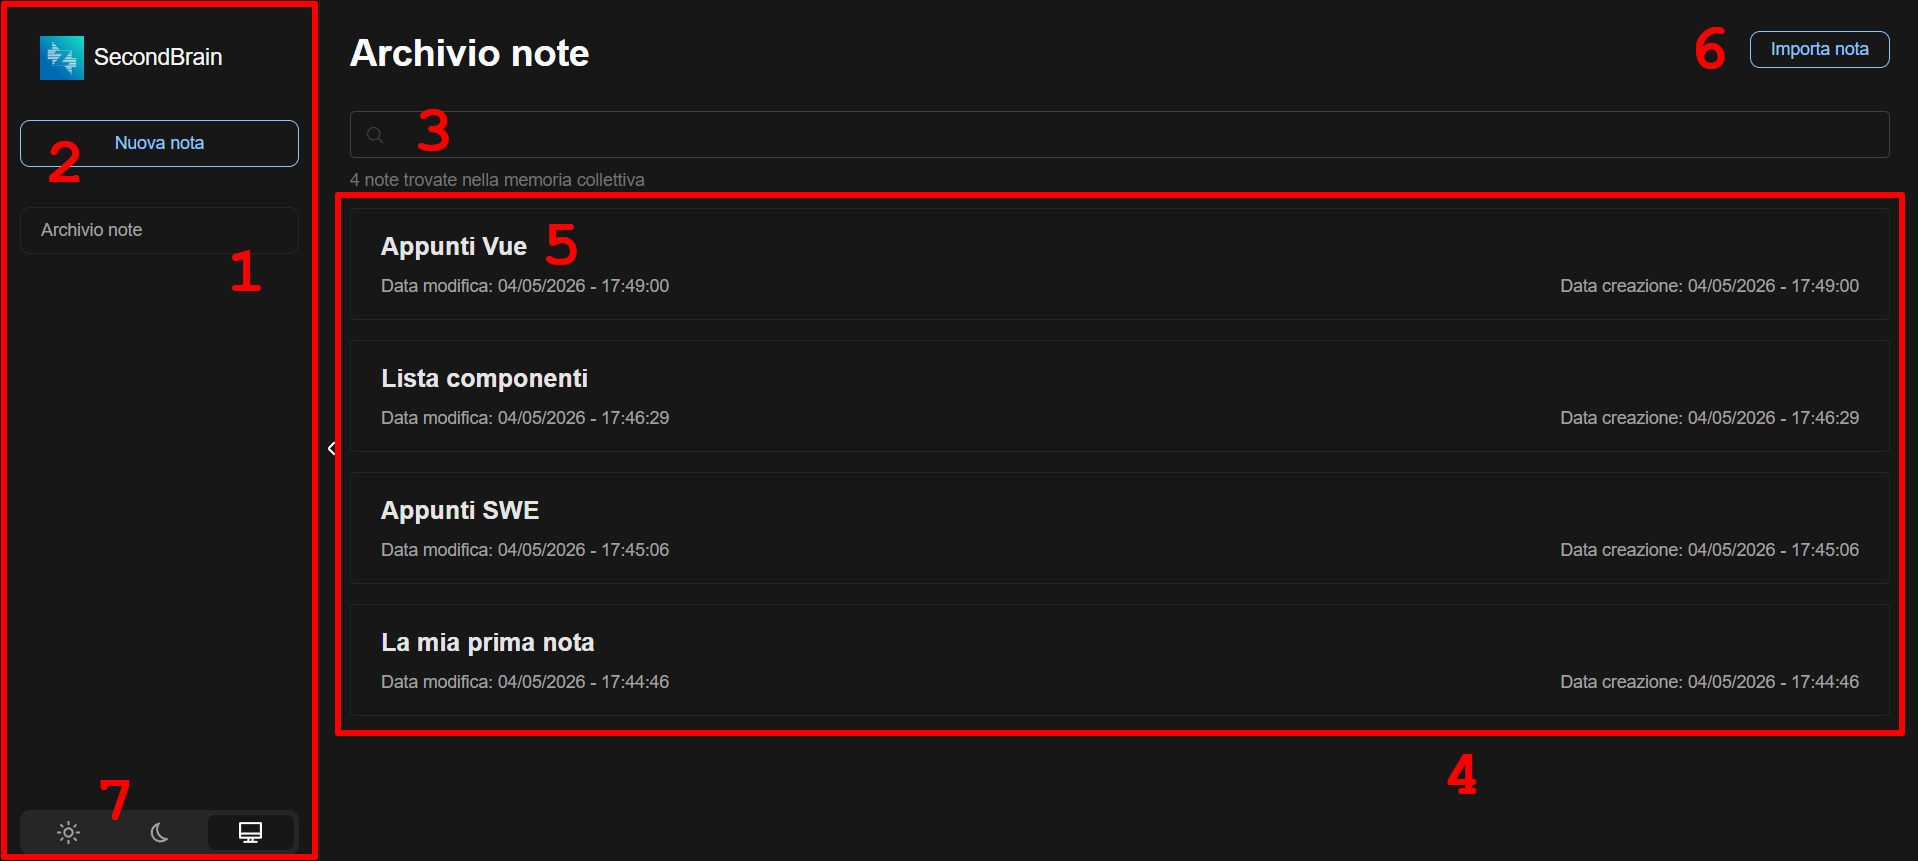
\includegraphics[width=1\textwidth]{resources/manual/archive/archivio.png}
    \caption{Schermata archivio note}
    \label{fig:archivio_note}
  \end{figure}
\end{center}

Questa schermata contiene:
\begin{enumerate}
  \item \textbf{Sidebar:} Permette all'utente di navigare fra le varie sezioni dell'applicazione, può essere nascosta o mostrata cliccando sulla freccia presente a sinistra.
  \item \textbf{Pulsante "Nuova nota":} Permette all'utente di creare una nuova nota in formato Markdown.
  \item \textbf{Barra di ricerca:} Permette all'utente di cercare una nota specifica all'interno dell'archivio, filtrando i risultati in tempo reale.
  \item \textbf{Elenco note:} Mostra tutte le note salvate all'interno dell'archivio. Ogni nota viene identificata univocamente dal sistema tramite il proprio titolo (non è quindi permessa la presenza di note con titolo identico; maggiori info nelle sezioni successive).
  \item \textbf{Nota singola:} Cliccando su una nota, è possibile visualizzarne il contenuto completo, modificarla o eliminarla.
  \item \textbf{Pulsante "Importa nota":} Permette all'utente di importare un file Markdown esterno, aggiungendolo all'archivio delle note.
  \item \textbf{Selettore tema:} Permette all'utente di selezionare il tema dell'applicazione tra: chiaro, scuro, sistema.
\end{enumerate}

Di seguito vengono presentate in dettaglio le funzionalità dell'archivio:

\subsubsection{Creazione Note}\label{subsubsec:nuova_nota}
Per creare una nota nuova è sufficiente cliccare sul relativo bottone \fcolorbox{black}{cyan!50}{Nuova nota} presente all'interno della SideBar (elemento \#2 nella \autoref{fig:archivio_note}). In seguito verrà aperto l'Editor di note con contenuto vuoto. (vedere \autoref{subsec:editor_note} per istruzioni dettagliate sull'Editor)

\subsubsection{Importazione Note}
SecondBrain permette anche la creazione di una nota attraverso l'importazione di un file locale in formato Markdown selezionato dall'utente. Per utilizzare tale funzione è sufficiente cliccare il relativo bottone \fcolorbox{black}{cyan!50}{Importa nota} (elemento \#6 nella \autoref{fig:archivio_note}) all'interno dell'archivio note. In seguito verrà aperta una finestra modale in cui selezionare il file desiderato:

\begin{center}
  \begin{figure}[H]
    \centering
    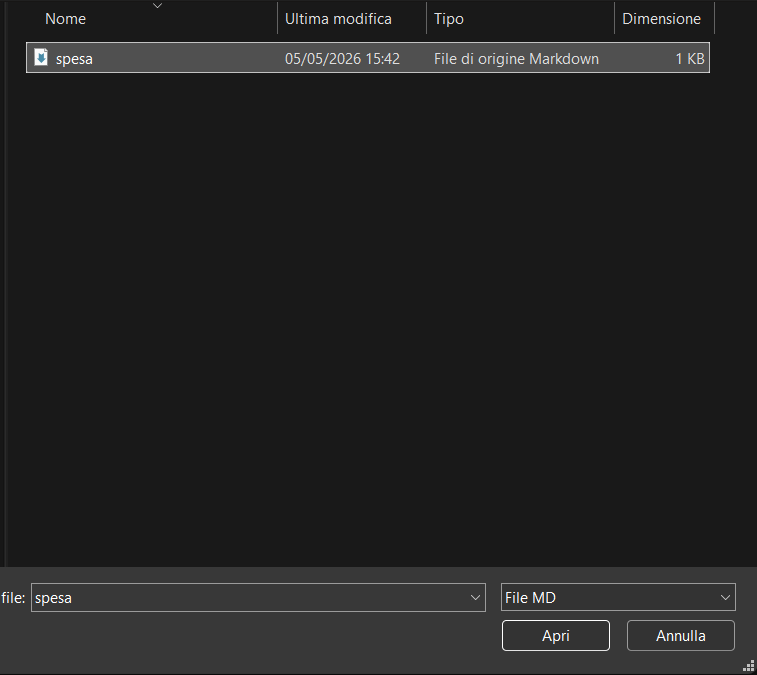
\includegraphics[width=0.45\textwidth]{resources/manual/archive/modale_import.png}
    \caption{Esempio finestra modale di selezione file (Windows 11)}
    \label{fig:modale_import}
  \end{figure}
\end{center}

Dopo aver selezionato il file e confermato l'azione il sistema provvederà ad effettuare l'importazione. Un avviso di successo notificherà l'utente dell'avvenuta creazione della nota nuova nell'archivio (il titolo è formato dal nome del file seguito dal dataora di importazione).

\begin{center}
  \begin{figure}[H]
    \centering
    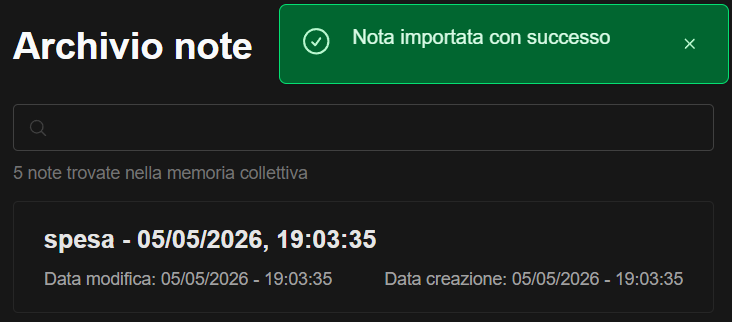
\includegraphics[width=0.4\textwidth]{resources/manual/archive/successo_import.png}
    \caption{Nota importata con relativo avviso di successo}
    \label{fig:successo_import}
  \end{figure}
\end{center}

Qualora si tentasse di importare un file con formato non supportato il sistema notificherà l'utente dell'errore senza proseguire ulteriormente con l'importazione:

\begin{center}
  \begin{figure}[H]
    \centering
    
\includegraphics[width=0.35\textwidth]{resources/manual/archive/errore_formato_import.png}
    \caption{Avviso di errore per formato non supportato}
    \label{fig:errore_formato_import}
  \end{figure}
\end{center}

\subsubsection{Apertura Note}\label{subsubsec:apertura_nota}
Cliccando con il tasto sinistro una delle note presenti nell'archivio (elemento \#5 nella \autoref{fig:archivio_note}) si aprirà l'Editor di note; al suo interno è possibile visualizzare e modificare il contenuto della nota. (vedere \autoref{subsec:editor_note} per istruzioni dettagliate sull'Editor)

\subsubsection{Ricerca Note}
Per effettuare una ricerca delle note in base al nome è sufficiente inserire il termine nella casella di ricerca (elemento \#3 nella \autoref{fig:archivio_note}) e premere "Invio".
La lista delle note verrà aggiornata con i risultati della ricerca.

\begin{center}
  \begin{figure}[H]
    \centering
    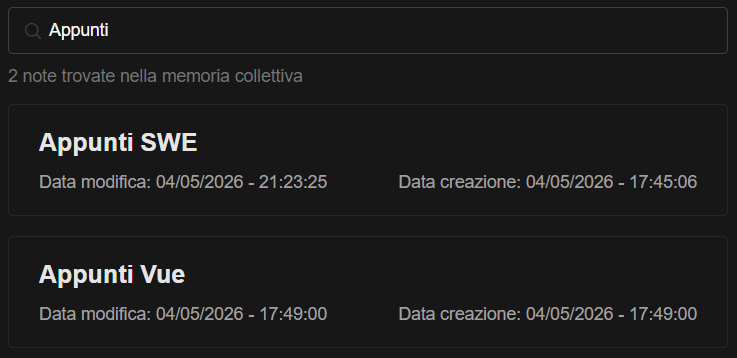
\includegraphics[width=0.6\textwidth]{resources/manual/archive/ricerca_archivio.png}
    \caption{Esempio di ricerca}
    \label{fig:ricerca_archivio}
  \end{figure}
\end{center}

\newpage

\subsubsection{Azioni contestuali}
Cliccando con il tasto destro su una nota all'interno dell'archivio (elemento \#5 nella \autoref{fig:archivio_note}), è possibile accedere al seguente menu contestuale:

\begin{center}
  \begin{figure}[H]
    \centering
    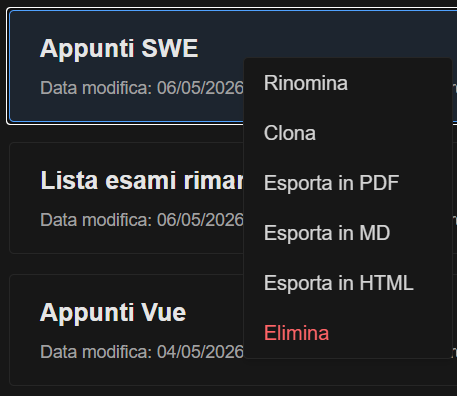
\includegraphics[width=0.4\textwidth]{resources/manual/archive/menu_context_nota_archivio.png}
    \caption{Menu contestuale nota in archivio}
    \label{fig:menu_contestuale}
  \end{figure}
\end{center}

\textbf{Le azioni possibili sono le seguenti:}

  \paragraph{\fcolorbox{black}{blue!15}{Rinominazione nota}}

    Cliccando sulla relativa opzione \fcolorbox{black}{cyan!50}{Rinomina} del menu contestuale (\autoref{fig:menu_contestuale}), l'utente può rinominare la nota selezionata attraverso la finestra modale visualizzata.
    
    \begin{center}
      \begin{figure}[H]
        \centering
        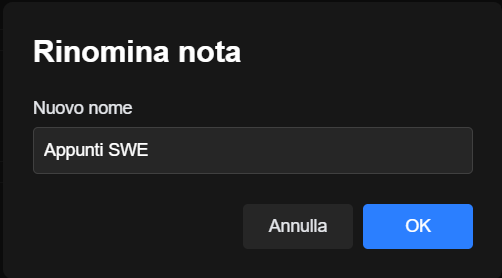
\includegraphics[width=0.4\textwidth]{resources/manual/archive/modale_rinomina_archivio.png}
        \caption{Finestra modale di rinominazione nota}
        \label{fig:modale_rinomina_archivio}
      \end{figure}
    \end{center}

    In seguito alla conferma da parte dell'utente viene effettuato un controllo di unicità del titolo: in caso di successo viene mostrato il relativo avviso di avvenuta rinominazione. 
    
    \begin{center}
      \begin{figure}[H]
        \centering
        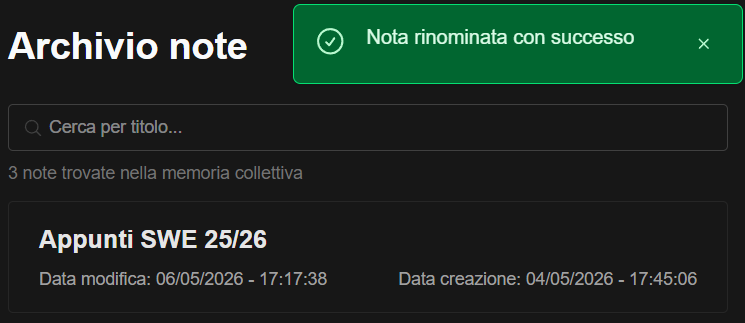
\includegraphics[width=0.5\textwidth]{resources/manual/archive/successo_rinomina_archivio.png}
        \caption{Nota rinominata con relativo avviso di successo}
        \label{fig:successo_rinomina_archivio}
      \end{figure}
    \end{center}

    In caso contrario viene visualizzato un messaggio di errore e la nota mantiene il titolo precedente.

    \begin{center}
      \begin{figure}[H]
        \centering
        
\includegraphics[width=0.35\textwidth]{resources/manual/archive/errore_titolo_rinomina_archivio.png}
        \caption{Avviso di errore titolo già in uso}
        \label{fig:errore_titolo_rinomina_archivio}
      \end{figure}
    \end{center}

  \paragraph{\fcolorbox{black}{blue!15}{Clonazione nota}}\label{par:clona_archivio}

    Cliccando sulla relativa opzione \fcolorbox{black}{cyan!50}{Clona} del menu contestuale (\autoref{fig:menu_contestuale}), l'utente può clonare la nota selezionata (creare una copia) attraverso la finestra modale visualizzata.
    Il sistema propone il titolo originale seguito dalla data e ora di clonazione come titolo per la nota clonata; l'utente può in ogni caso personalizzarlo. 

    \begin{center}
      \begin{figure}[H]
        \centering
        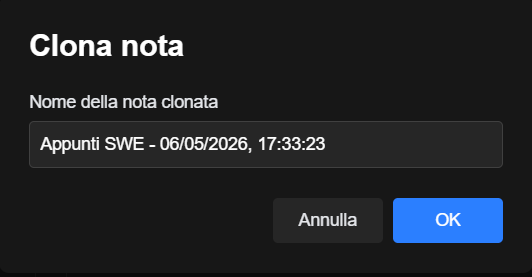
\includegraphics[width=0.4\textwidth]{resources/manual/archive/modale_clona_archivio.png}
        \caption{Finestra modale di clonazione nota}
        \label{fig:modale_clona_archivio}
      \end{figure}
    \end{center}

    Dopo la conferma il sistema effettua un controllo di unicità del titolo; in caso di successo viene mostrato il relativo avviso di avvenuta clonazione.
    
    \begin{center}
      \begin{figure}[H]
        \centering
        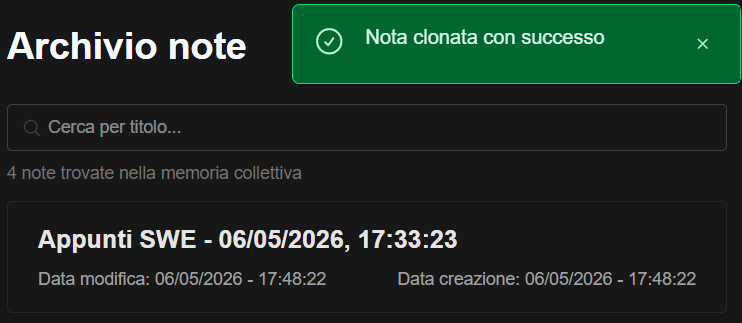
\includegraphics[width=0.5\textwidth]{resources/manual/archive/successo_clona_archivio.png}
        \caption{Nota clonata con relativo avviso di successo}
        \label{fig:successo_clona_archivio}
      \end{figure}

      In caso di titolo già utilizzato viene visualizzato un messaggio di errore (vedi \autoref{fig:errore_titolo_rinomina_archivio}).

    \end{center}

\vspace{2cm}

\newpage

  \paragraph{\fcolorbox{black}{blue!15}{Esportazione nota}}\label{par:esporta_archivio}

    L'utente può esportare una nota presente in archivio in uno dei seguenti formati:
        \begin{itemize}
          \item PDF
          \item Markdown
          \item HTML
        \end{itemize}
    Cliccando su una delle opzioni \fcolorbox{black}{cyan!50}{Esporta} del menu contestuale (\autoref{fig:menu_contestuale}), il sistema fornirà al browser un file nel formato selezionato; un avviso notificherà l'utente del successo dell'esportazione ed automaticamente verrà avviato il download del file.
    
    \begin{center}
      \begin{figure}[H]
        \centering
        
\includegraphics[width=0.4\textwidth]{resources/manual/archive/successo_esporta_archivio.png}
        \caption{Avviso di successo esportazione}
        \label{fig:successo_esportazione}
      \end{figure}

      \begin{figure}[H]
        \centering
        
\includegraphics[width=0.3\textwidth]{resources/manual/archive/esempio_download_esporta_pdf.png}
        
\includegraphics[width=0.3\textwidth]{resources/manual/archive/esempio_download_esporta_md.png}
        
\includegraphics[width=0.3\textwidth]{resources/manual/archive/esempio_download_esporta_html.png}
        \caption{Esempi di file generati dall'esportazione nei vari formati (Windows 11)}
        \label{fig:esempio_file_esportazione}
      \end{figure}
    \end{center}

  \paragraph{\fcolorbox{black}{red!20}{Eliminazione nota}}

    Cliccando sulla relativa opzione \fcolorbox{black}{red!40}{Elimina} del menu contestuale (\autoref{fig:menu_contestuale}), l'utente può eliminare la nota selezionata. Viene mostrata una finestra modale di conferma:

    \begin{center}
      \begin{figure}[H]
        \centering
        
\includegraphics[width=0.5\textwidth]{resources/manual/archive/modale_elimina.png}
        \caption{Finestra modale di eliminazione nota}
        \label{fig:modale_elimina}
      \end{figure}
    \end{center}

    In caso si confermi l'azione, la nota verrà rimossa in modo definitivo e verrà visualizzato un messaggio di avvenuta eliminazione.

    \begin{center}
      \begin{figure}[H]
        \centering
        
\includegraphics[width=0.4\textwidth]{resources/manual/archive/successo_elimina.png}
        \caption{Avviso di avvenuta eliminazione}
        \label{fig:successo_elimina}
      \end{figure}
    \end{center}

\newpage

\subsection{Editor Note}\label{subsec:editor_note}
Creando una nota nuova (vedi sezione \ref{subsubsec:nuova_nota}) oppure aprendo una delle note presenti nell'archivio (vedi sezione \ref{subsubsec:apertura_nota}) si accede all'editor di note. Al suo interno è possibile visualizzare e modificare il contenuto della nota.

  \begin{center}
    \begin{figure}[H]
      \centering
      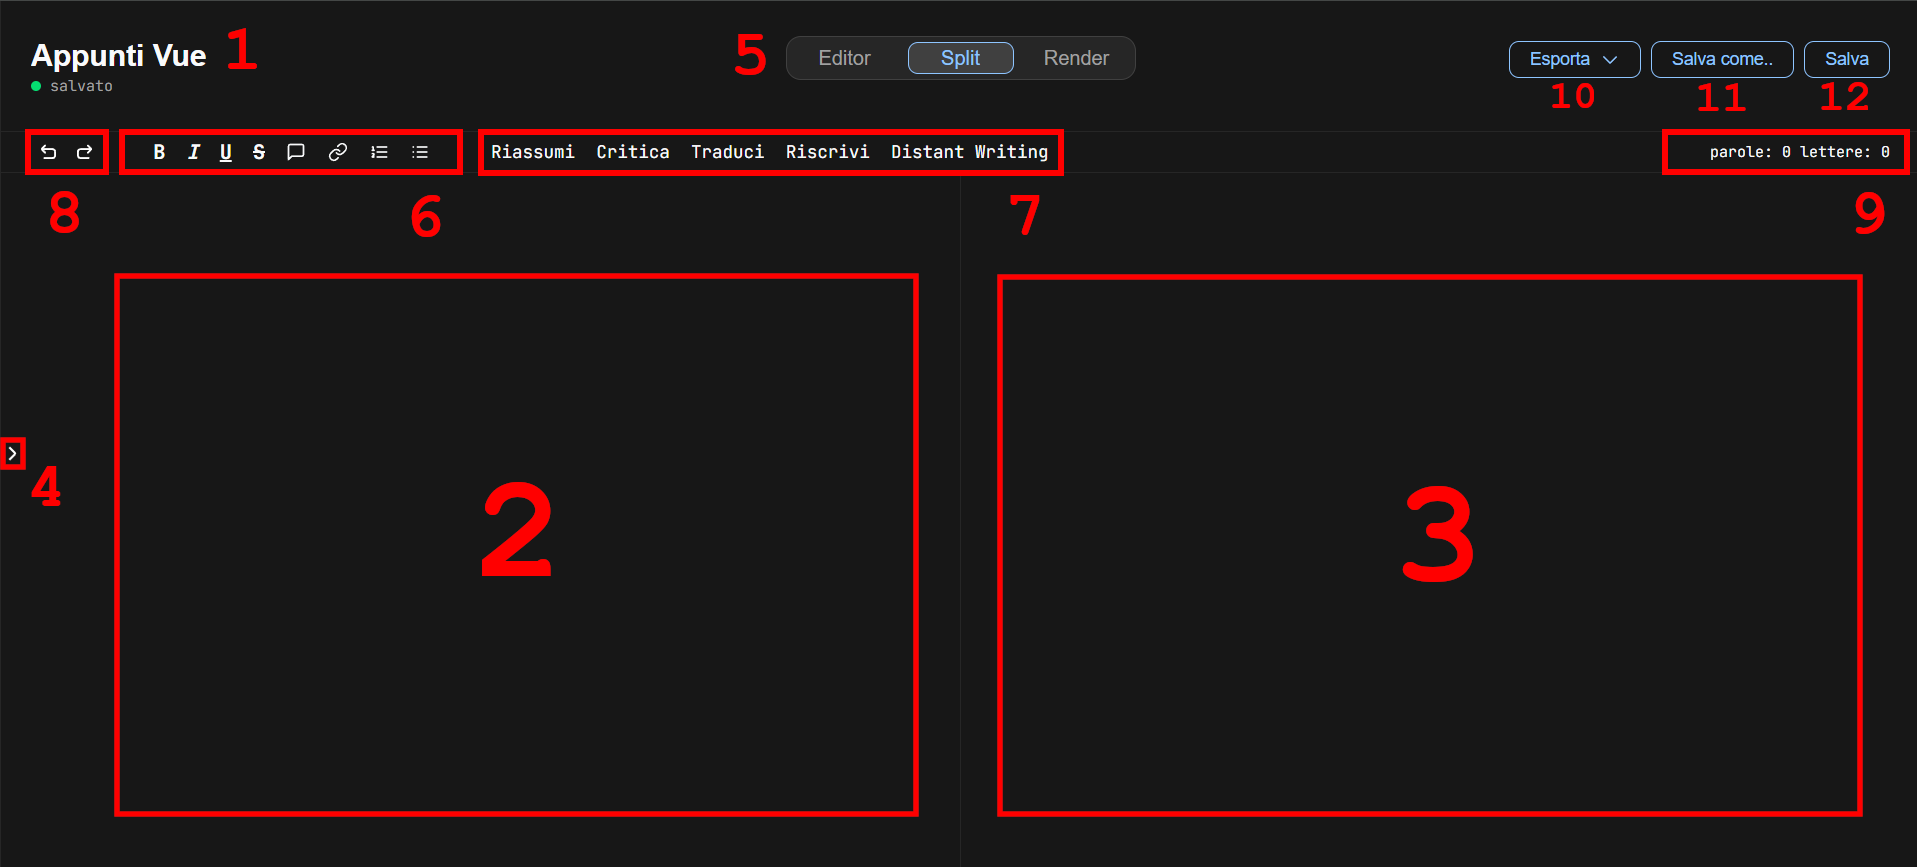
\includegraphics[width=1\textwidth]{resources/manual/editor/editor.png}
      \caption{Schermata editor note}
      \label{fig:editor_note}
    \end{figure}
  \end{center}

Questa schermata contiene:
\begin{enumerate}
  \item \textbf{Titolo Nota:} il nome della nota è visualizzato assieme ad un indicatore dello stato di salvataggio.
  \item \textbf{Area di modifica:} sezione in cui l'utente può scrivere e modificare il contenuto della nota, usufruendo anche delle altre funzionalità di supporto fornite dall'editor.
  \item \textbf{Area di rendering:} sezione in cui viene visualizzato il contenuto presente nell'area di modifica formattato secondo la sintassi Markdown.
  \item \textbf{Pulsante Sidebar:} pulsante con cui si accede alla barra di navigazione laterale.
  \item \textbf{Selettore Visualizzazione:} permette all'utente di selezionare il layout dell'editor in base alle proprie esigenze.
  \item \textbf{Barra formattazione testo:} contiene i pulsanti tramite cui vengono applicati i relativi stili al testo selezionato tramite marcatori di sintassi Markdown.
  \item \textbf{Barra azioni IA:} contiene i pulsanti con cui si possono eseguire azioni IA per applicare modifiche al contenuto della nota.
  \item \textbf{Pulsanti UNDO-REDO:} permettono all'utente di annullare l'ultimo comando eseguito o ripetere l'ultimo comando annullato. 
  \item \textbf{Contatore caratteri:} un indicatore che tiene conto del numero totale di lettere e parole all'interno della nota.
  \item \textbf{Pulsante "Esporta":} permette di eseguire l'esportazione della nota aperta.
  \item \textbf{Pulsante "Salva con nome":} realizza in archivio una copia della nota aperta ed aggiorna la schermata dell'editor con la copia creata. 
  \item \textbf{Pulsante "Salva":} esegue il salvataggio della nota aperta, aggiornandone il contenuto all'interno dell'archivio.
\end{enumerate}

Di seguito vengono presentate in dettaglio le funzionalità fornite all'interno dell'editor.

  \subsubsection{Accesso barra di navigazione}

  Premendo il pulsante \fcolorbox{black}{white}{\textbf{\textgreater}} (elemento \#4 nella \autoref{fig:editor_note}) si apre la barra di navigazione da cui si può accedere alle varie sezioni dell'applicazione.

  \begin{center}
    \begin{figure}[H]
      \centering
      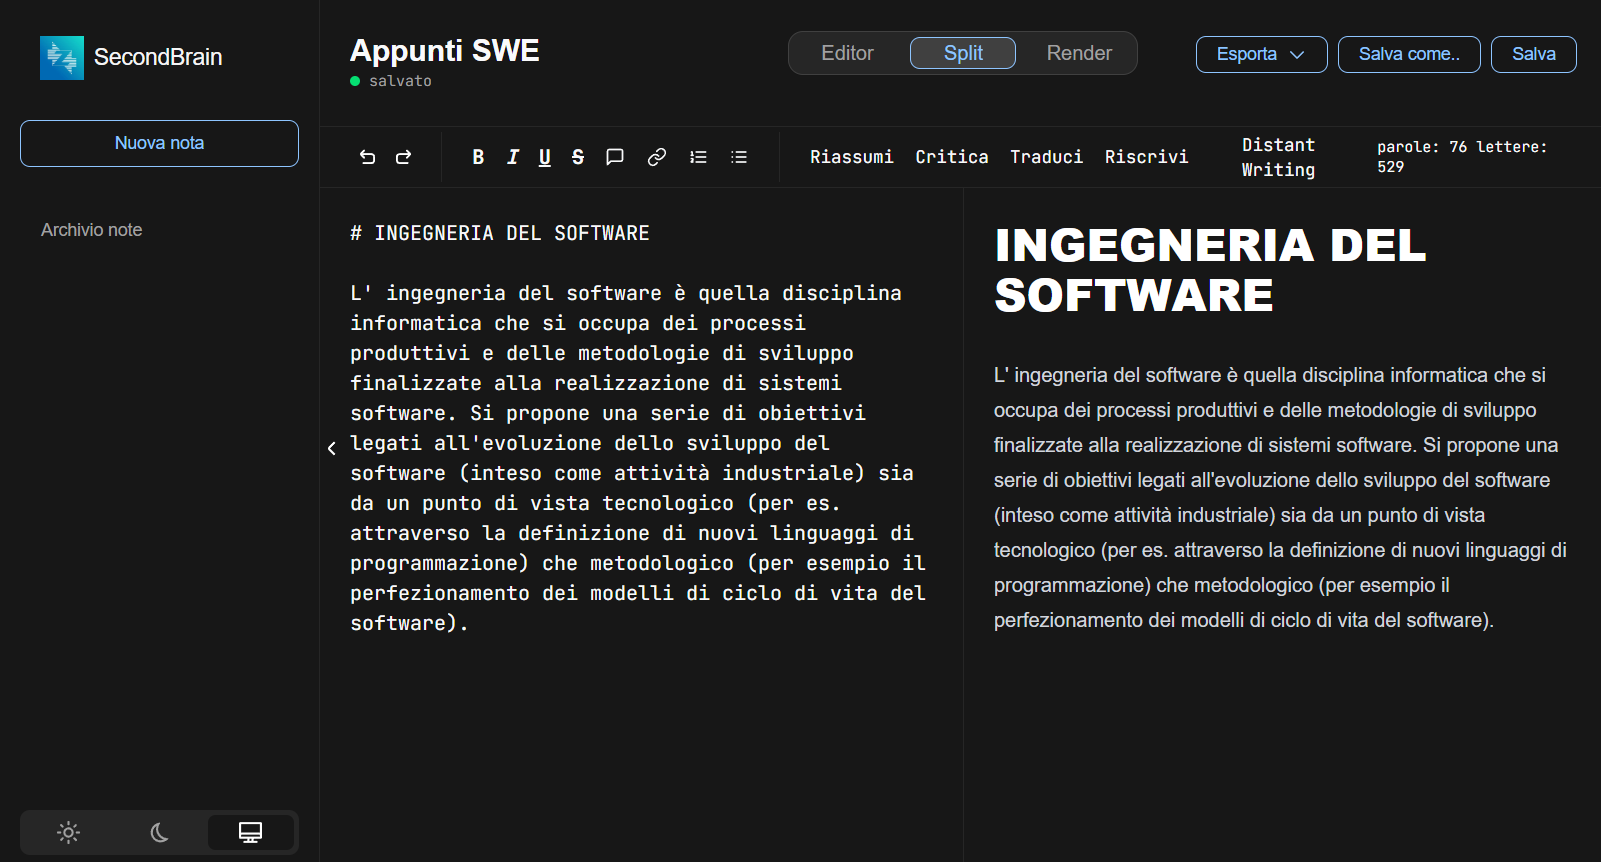
\includegraphics[width=0.8\textwidth]{resources/manual/editor/navbar_editor.png}
      \caption{Sidebar accessibile dall'editor}
      \label{fig:sidebar_editor}
    \end{figure}
  \end{center}

  \subsubsection{Layout visualizzazione}\label{subsubsec:selettore_layout}
  Tramite il selettore di layout (elemento \#5 nella \autoref{fig:editor_note}), l'utente può modificare la visualizzazione delle aree di lavoro. Si può scegliere tra: \fcolorbox{black}{cyan!30}{Editor} (solo area di modifica), \fcolorbox{black}{cyan!30}{Render} (solo area di rendering) o \fcolorbox{black}{cyan!30}{Split} (entrambe le aree). Il layout di default è impostato su \texttt{Split}.

  \begin{center}
    \begin{figure}[H]
      \centering
      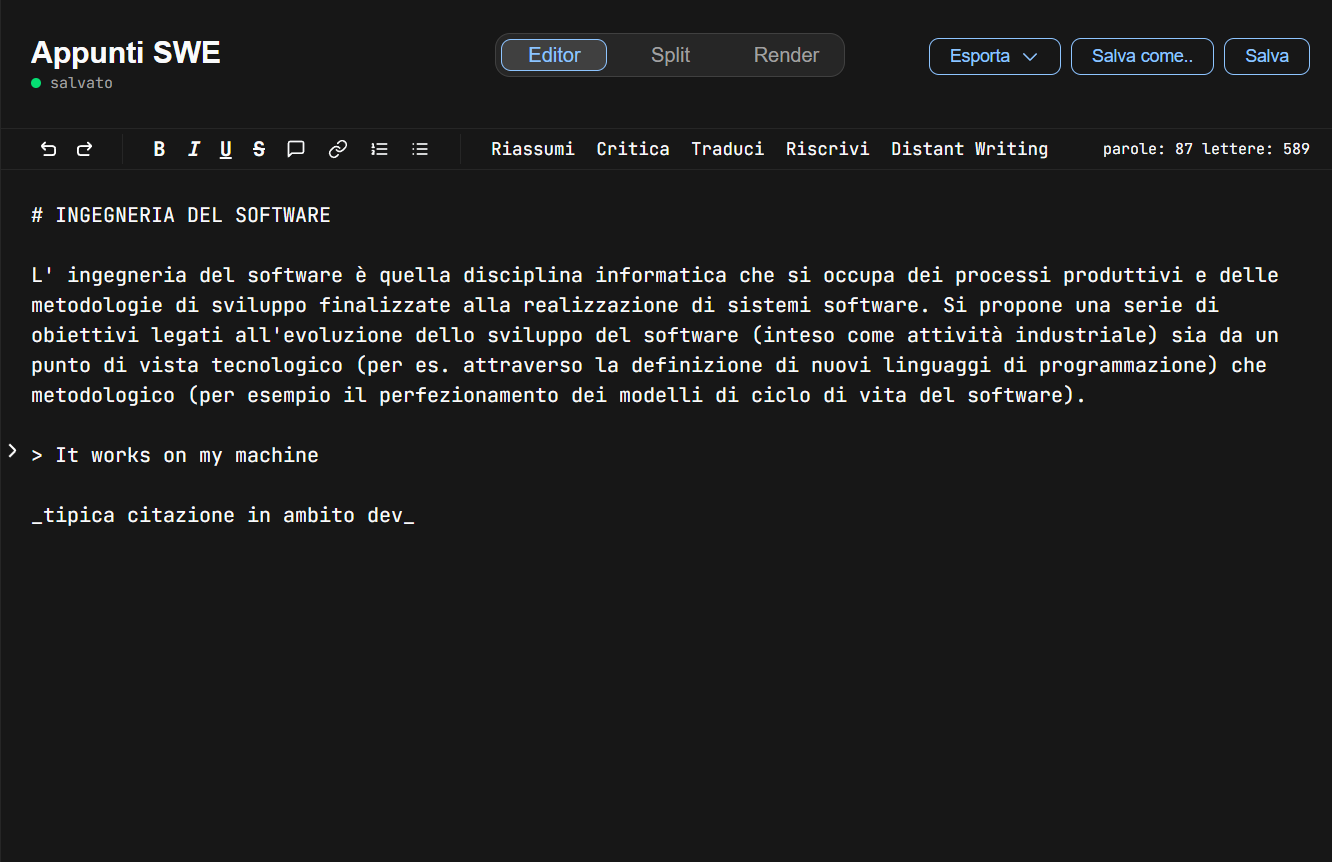
\includegraphics[width=0.31\textwidth]{resources/manual/editor/editor_layout.png}
      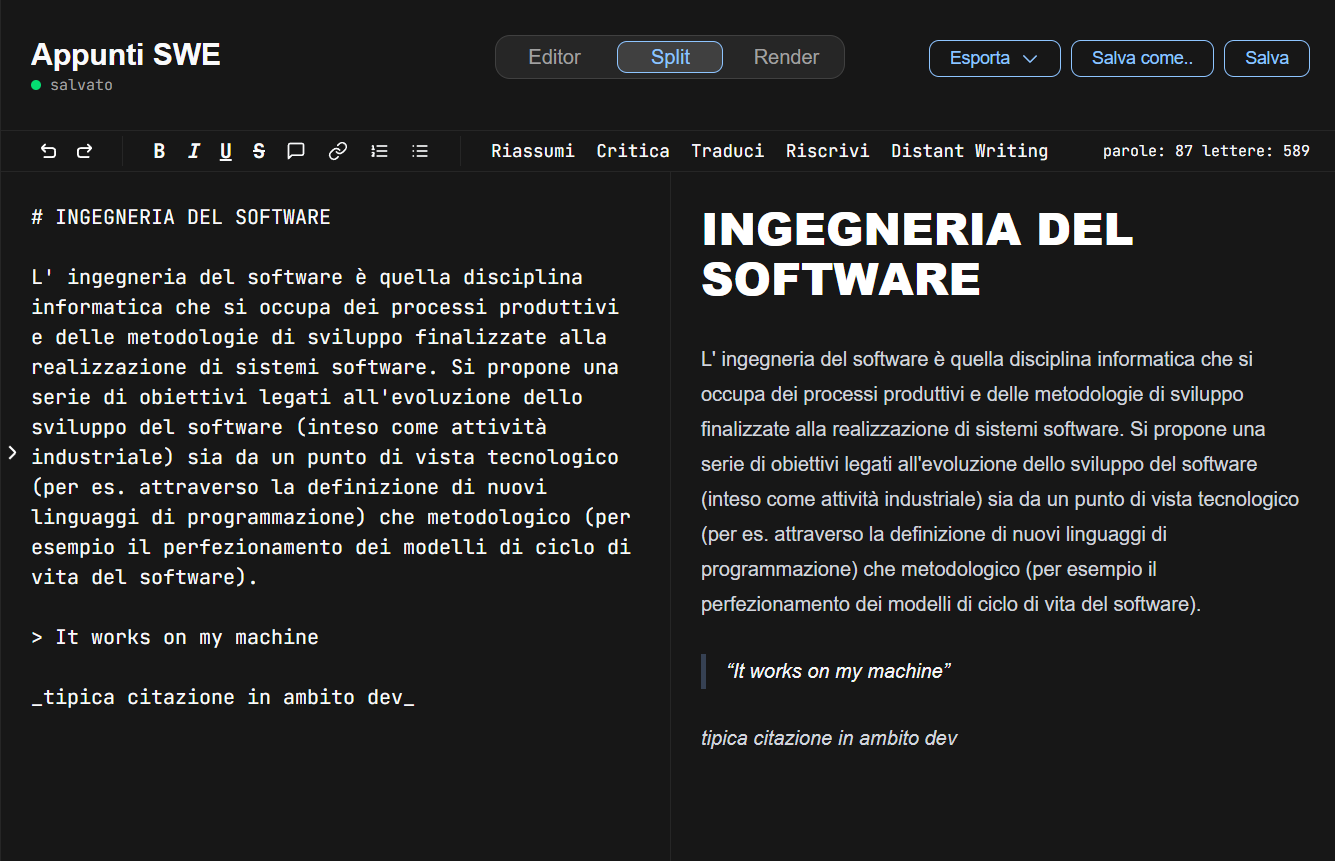
\includegraphics[width=0.31\textwidth]{resources/manual/editor/split_layout.png}
      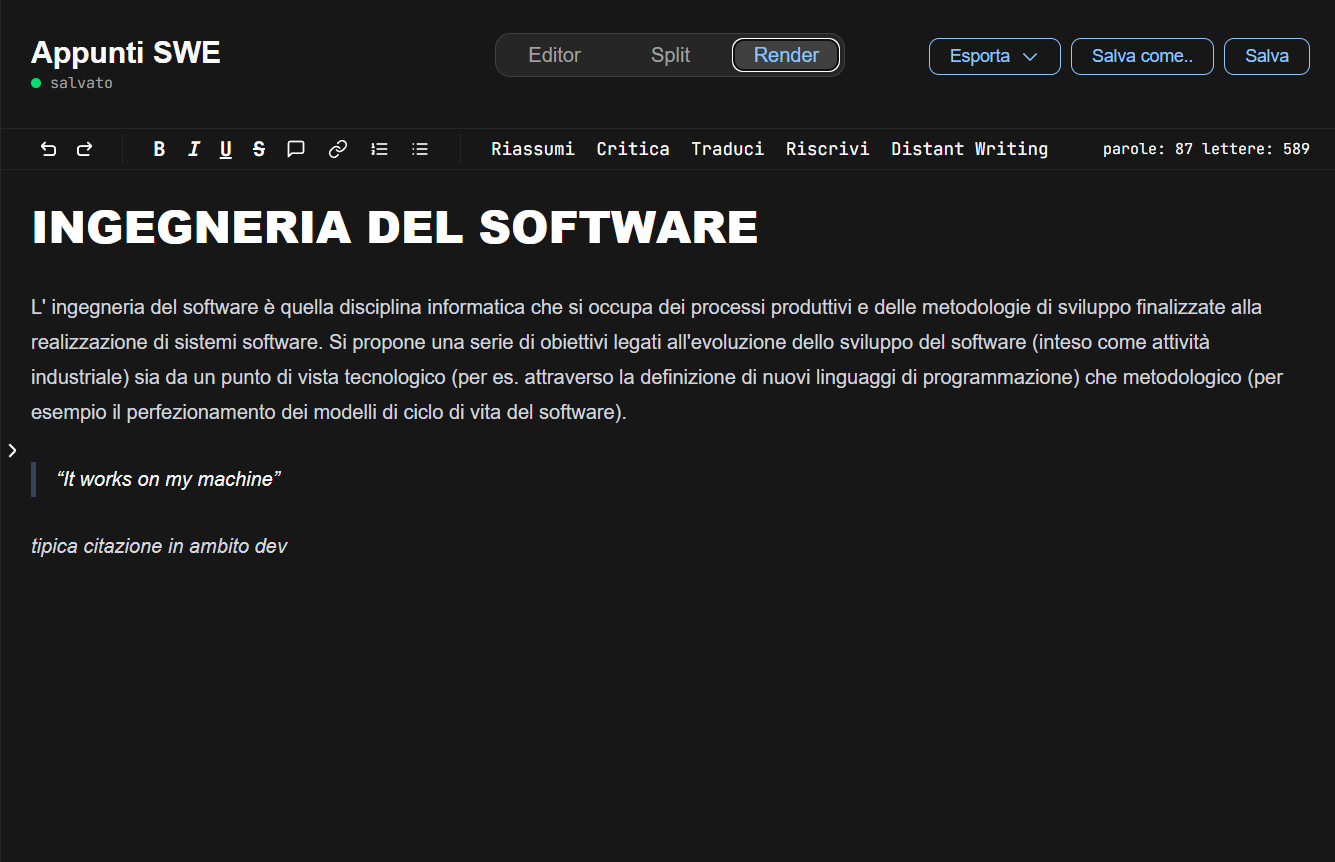
\includegraphics[width=0.31\textwidth]{resources/manual/editor/render_layout.png}
      \caption{Layout di visualizzazione disponibili}
      \label{fig:layouts_editor}
    \end{figure}
  \end{center}

  \subsubsection{Scrittura contenuto}

  L'utente può lavorare al contenuto della nota all' interno dell'area di modifica (elemento \#2 nella \autoref{fig:editor_note}). È possibile aggiungere manualmente marcatori di sintassi Markdown oppure usufruire dei bottoni presenti nella barra degli stili di testo (elemento \#6 nella \autoref{fig:editor_note}), la quale offre le seguenti formattazioni (componibili fra loro):
      \begin{itemize}
        \item \texttt{Grassetto | Corsivo | Sottolineato | Barrato}
        \item \texttt{Commento | Link}
        \item \texttt{Elenco Numerato | Elenco Puntato}
      \end{itemize}

  \begin{center}
    \begin{figure}[H]
      \centering
      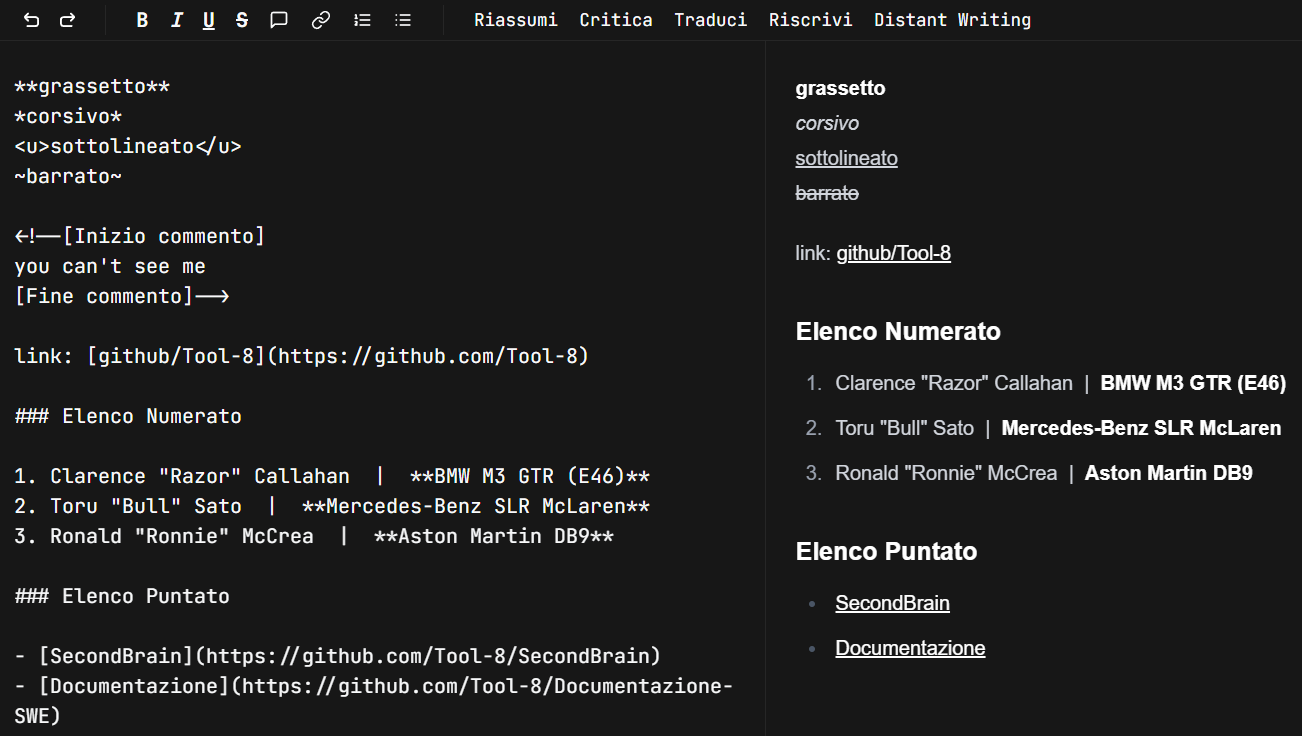
\includegraphics[width=0.9\textwidth]{resources/manual/editor/esempio_stili_md.png}
      \caption{Esempio formattazioni applicabili tramite barra degli stili (in ordine da sx a dx)}
      \label{fig:esempio_stili_md}
    \end{figure}
  \end{center}

  \textbf{ATTENZIONE: È necessario selezionare del testo per l'applicazione di stile tramite i pulsanti, in caso contrario l'utente verrà avvisato della mancata selezione.}

  \begin{center}
    \begin{figure}[H]
      \centering
      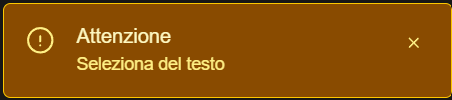
\includegraphics[width=0.4\textwidth]{resources/manual/editor/warning_seleziona_testo.png}
      \caption{Avviso di mancata selezione testo}
      \label{fig:warning_seleziona_testo}
    \end{figure}
  \end{center}

  Tramite il selettore di layout (vedi sezione \ref{subsubsec:selettore_layout}), è possibile nascondere o meno l'area di modifica.

  \subsubsection{Visualizzazione contenuto formattato}

  Il contenuto presente nell'area di modifica (elemento \#2 nella \autoref{fig:editor_note}) viene visualizzato in maniera formattata all'interno dell'area di rendering (elemento \#3 nella \autoref{fig:editor_note}). La formattazione si aggiorna in tempo reale reagendo ad ogni modifica del contenuto, senza bisogno di azioni manuali da parte dell'utente. Tramite il selettore di layout (vedi sezione \ref{subsubsec:selettore_layout}), è possibile nascondere o meno l'area di visualizzazione formattata.


  \subsubsection{Funzionalità IA}

  L'utente può avvalersi del supporto di un LLM per modificare il contenuto della nota; è sufficiente selezionare parte del testo, o la sua interezza, e premere uno dei pulsanti disponibili nella barra di funzioni IA (elemento \#7 nella \autoref{fig:editor_note}).
  Successivamente, verrà aperta la sezione riguardante l'interazione con l'LLM. All'interno è possibile visualizzare il testo selezionato, il bottone di esecuzione ed il risultato (inizialmente vuoto).
  Una volta premuto il bottone di esecuzione (definito col nome dell'azione) il sistema comunicherà con l'LLM e ritornerà il risultato generato. 
  In fondo sono presenti i pulsanti per aggiungere automaticamente il risultato al contenuto della nota, in relazione alla posizione del testo selezionato: \texttt{prima}, \texttt{dopo}, \texttt{sostituisci}, \texttt{in fondo alla pagina}. Eventualmente è anche possibile copiare il risultato nella clipboard per gestirlo manualmente.

  \begin{center}
    \begin{figure}[H]
      \centering
      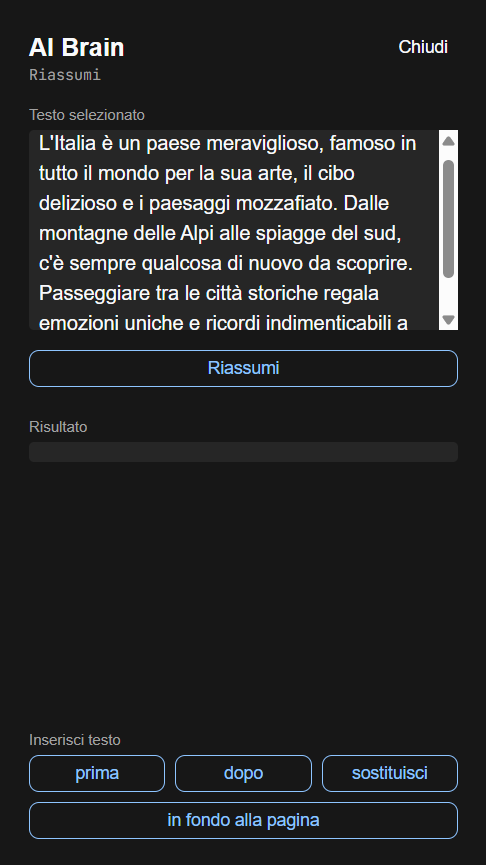
\includegraphics[width=0.4\textwidth]{resources/manual/editor/aside_riassumi.png}
      \hspace{1cm}
      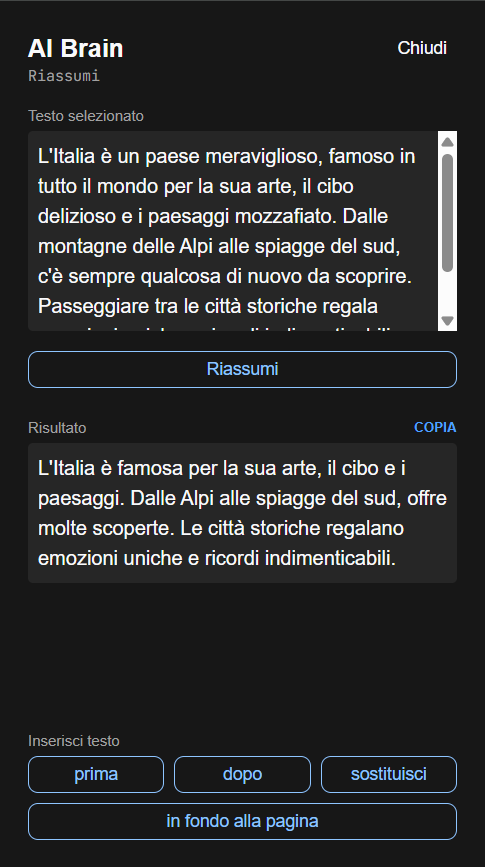
\includegraphics[width=0.4\textwidth]{resources/manual/editor/aside_riassumi_risultato.png}
      \caption{Esempio di pre e post esecuzione azione IA (riassunto)}
      \label{fig:aside_riassumi}
    \end{figure}
  \end{center}

  Per utilizzare le funzioni IA è necessario selezionare del testo, in caso contrario verrà visualizzato un avviso della mancata selezione.

  \begin{center}
    \begin{figure}[H]
      \centering
      
\includegraphics[width=0.4\textwidth]{resources/manual/editor/warning_seleziona_testo_ai.png}
      \caption{Avviso di testo non selezionato}
      \label{fig:avviso_seleziona_testo_ia}
    \end{figure}
  \end{center}

  In caso vi siano degli errori durante l'esecuzione, viene mostrato un avviso all'utente con la descrizione della causa.

  \begin{center}
    \begin{figure}[H]
      \centering
      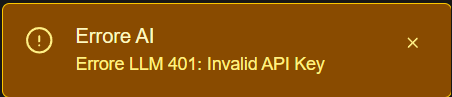
\includegraphics[width=0.4\textwidth]{resources/manual/editor/warning_ai_api_key.png}
      \caption{Esempio di avviso errore causa chiave API non valida}
      \label{fig:avviso_errore_ia}
    \end{figure}
  \end{center}

  Una volta inserito all'interno dell'area di modifica, il risultato dell'interazione IA ed il testo di input (se non sostituito) verranno evidenziati (non influisce sul rendering):

  \begin{center}
    \begin{figure}[H]
      \centering
      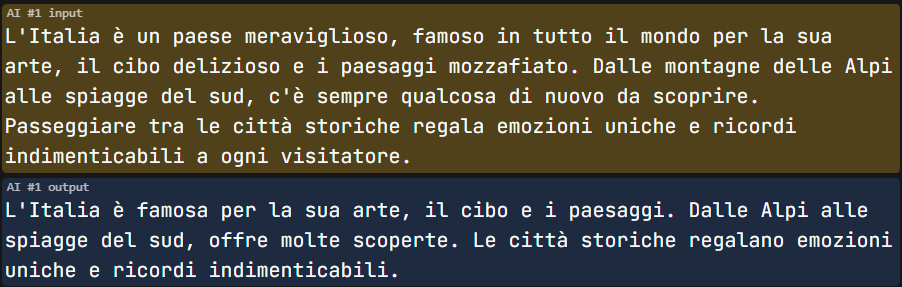
\includegraphics[width=0.7\textwidth]{resources/manual/editor/input_output_ia_evidenziato.png}
      \caption{Input e Output della funzione IA evidenziati nell'area di modifica}
      \label{fig:evidenzia_output_ia}
    \end{figure}
  \end{center}

  Se in qualche momento l'utente modifica l'output di un'azione IA, il sistema mostra un avviso all'utente:
  
  \begin{center}
    \begin{figure}[H]
      \centering
      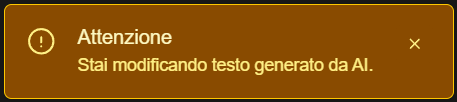
\includegraphics[width=0.4\textwidth]{resources/manual/editor/warning_modifica_ai.png}
      \caption{Avviso di modifica output azione IA}
      \label{fig:avviso_modifica_ia}
    \end{figure}
  \end{center}  
  
  \textbf{Le azioni possibili sono le seguenti:}

  \paragraph{\fcolorbox{black}{blue!15}{Riassumi}}

    Cliccando sul relativo bottone \fcolorbox{black}{cyan!50}{Riassumi}, verrà aperta la finestra di interazione LLM (vedi esempio in \autoref{fig:aside_riassumi}) configurata per generare un riassunto del testo selezionato. Il resto dell'esecuzione rimane uguale alle altre azioni.
    
  \paragraph{\fcolorbox{black}{blue!15}{Critica}}

    Cliccando sul relativo bottone \fcolorbox{black}{cyan!50}{Critica}, verrà aperta la finestra di interazione LLM (vedi esempio in \autoref{fig:aside_riassumi}) configurata per generare una critica del testo selezionato seguendo la metafora dei \textit{"Sei cappelli per pensare"} di \textit{Edward de Bono}. All'interno della finestra si potrà infatti selezionare tra 6 diversi tipi di critica: 
    \begin{itemize}
      \item \textbf{Cappello bianco}: riguarda fatti, dati e informazioni oggettive.
      \item \textbf{Cappello rosso}:  esprime emozioni, sentimenti e intuizioni.
      \item \textbf{Cappello nero}: evidenzia rischi, problemi e aspetti critici.
      \item \textbf{Cappello giallo}: si focalizza sugli aspetti positivi e sui benefici.
      \item \textbf{Cappello verde}: stimola la creatività, le nuove idee e le soluzioni alternative.
      \item \textbf{Cappello blu}: controlla l’andamento del lavoro, verificando che la discussione segua un metodo ordinato. 
    \end{itemize}
    
    \begin{center}
      \begin{figure}[H]
      \centering
      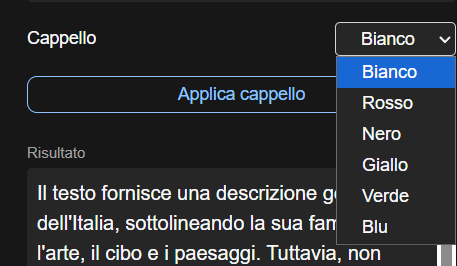
\includegraphics[width=0.4\textwidth]{resources/manual/editor/select_critica.png}
      \caption{Selezione "cappello" all'interno della finestra di interazione IA}
      \label{fig:select_critica}
    \end{figure}
    \end{center}

    Il resto dell'esecuzione rimane uguale alle altre azioni.

  \paragraph{\fcolorbox{black}{blue!15}{Traduci}}

    Cliccando sul relativo bottone \fcolorbox{black}{cyan!50}{Traduci}, verrà aperta la finestra di interazione LLM (vedi esempio in \autoref{fig:aside_riassumi}) configurata per generare la traduzione del testo selezionato in una tra le lingue supportate: 
    \begin{itemize}
      \item Italiano 
      \item Inglese (selezionata di default)
      \item Francese
      \item Tedesco
      \item Spagnolo
    \end{itemize}

    \begin{center}
      \begin{figure}[H]
      \centering
      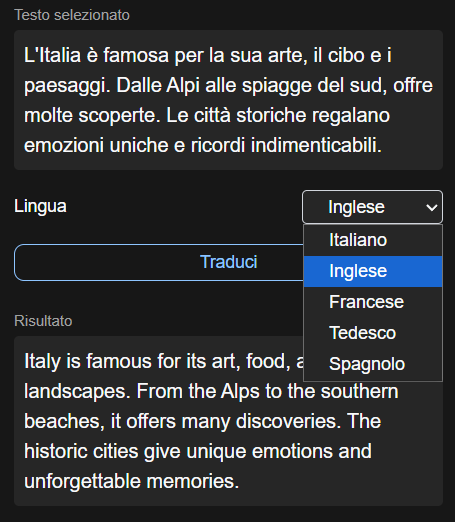
\includegraphics[width=0.4\textwidth]{resources/manual/editor/select_traduci.png}
      \caption{Selezione lingua all'interno della finestra di interazione IA}
      \label{fig:select_traduci}
      \end{figure}
    \end{center}

    Qualora si andasse a modificare il testo originale da cui è stata generata una traduzione, all'interno di quest'ultima verrà reso disponibile un pulsante di \textit{Ritraduzione} con cui effettuare un aggiornamento automatico sulla base del testo modificato dall'utente.

    \begin{center}
      \begin{figure}[H]
      \centering
      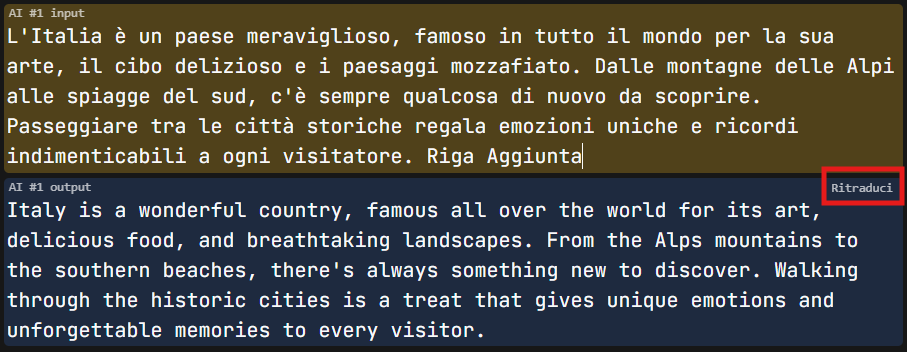
\includegraphics[width=0.7\textwidth]{resources/manual/editor/bottone_ritraduci.png}
      \caption{Bottone ritraduci all'interno della traduzione}
      \label{fig:bottone_ritraduci}
      \end{figure}
    \end{center}
  
    Il resto dell'esecuzione rimane uguale alle altre azioni.

  \paragraph{\fcolorbox{black}{blue!15}{Riscrivi}}

    Cliccando sul relativo bottone \fcolorbox{black}{cyan!50}{Riscrivi}, verrà aperta la finestra di interazione LLM (vedi esempio in \autoref{fig:aside_riassumi}) configurata per riscrivere il testo selezionato migliorando uno o più tra i seguenti aspetti (è obbligatorio sceglierne almeno uno):
    \begin{itemize}
      \item \textbf{Grammatica}: corregge errori e migliora la correttezza sintattica del testo.
      \item \textbf{Estensione}: amplia il testo aggiungendo dettagli, spiegazioni o esempi, mantenendo il significato originale.
      \item \textbf{Lessico}: migliora la scelta delle parole, sostituendo termini semplici o ripetitivi con alternative migliori.
      \item \textbf{Stile}: rielabora il tono e la forma del testo, rendendolo più efficace.
    \end{itemize} 

    \begin{center}
      \begin{figure}[H]
      \centering
      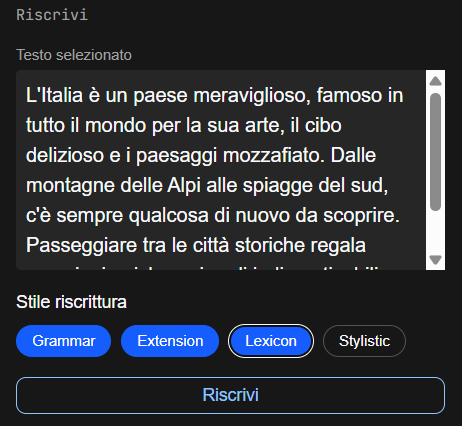
\includegraphics[width=0.4\textwidth]{resources/manual/editor/select_riscrivi.png}
      \caption{Selezione aspetti di riscrittura all'interno della finestra di interazione IA}
      \label{fig:select_riscrivi}
      \end{figure}
    \end{center}

    Il resto dell'esecuzione rimane uguale alle altre azioni.
  
  \paragraph{\fcolorbox{black}{blue!15}{Distant Writing}}

    Cliccando sul relativo bottone \fcolorbox{black}{cyan!50}{Distant Writing},  verrà aperta la finestra di interazione LLM (vedi esempio in \autoref{fig:aside_riassumi}) configurata per generare un testo nuovo usando come descrizione il testo selezionato dall'utente. Il resto dell'esecuzione rimane uguale alle altre azioni.
    
  \subsubsection{Funzioni Undo-Redo}

  Le modifiche effettuate al contenuto della nota vengono tracciate in modo da permettere all'utente di ripristinare o annullare rapidamente tali modifiche.
  I due pulsanti presenti nella barra in alto a sinistra (elemento \#8 nella \autoref{fig:editor_note}) servono rispettivamente per:
    \begin{itemize}
      \item \textbf{UNDO:} annullare l'ultima modifica eseguita dall'utente. È possibile eseguire molteplici \texttt{UNDO} in successione fino alla prima modifica registrata. 
      \item \textbf{REDO:} ripristinare l'effetto generato da un'azione di \texttt{UNDO}. È possibile eseguire molteplici \texttt{REDO} finché non si ripristina il contenuto all'ultima modifica eseguita.
    \end{itemize}

    \begin{center}
    \begin{figure}[H]
      \centering
      
\includegraphics[width=0.2\textwidth]{resources/manual/editor/UNDO-REDO.png}
      \caption{Pulsanti rispettivamente per UNDO e REDO}
      \label{fig:UNDO_REDO}
    \end{figure}
  \end{center}

  Le azioni di UNDO e REDO possono essere eseguite in modo alternato permettendo di "ripercorrere" in avanti o indietro le modifiche al contenuto.

  \subsubsection{Salvataggio Nota}

  Per salvare le modifiche eseguite al contenuto della nota è sufficiente premere il bottone \fcolorbox{black}{blue!30}{Salva} (elemento \#12 nella \autoref{fig:editor_note}). Assieme al contenuto è anche possibile rinominare la nota sempre attraverso l'azione di salvataggio; basterà cliccare sul titolo, il quale diventerà modificabile:

  \begin{center}
    \begin{figure}[H]
      \centering
      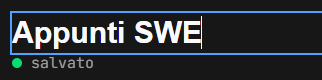
\includegraphics[width=0.38\textwidth]{resources/manual/editor/titolo_pre_rinomina.png}
      
\includegraphics[width=0.4\textwidth]{resources/manual/editor/titolo_post_rinomina.png}
      \caption{Esempio di modifica titolo}
      \label{fig:esempio_rinomina_titolo}
    \end{figure}
  \end{center}

  Una volta modificato il titolo è sufficiente premere il bottone di salvataggio.
  Il sistema effettuerà un controllo di unicità del titolo nuovo e in caso di successo aggiornerà titolo e contenuto della nota.

  \begin{center}
    \begin{figure}[H]
      \centering
      
\includegraphics[width=0.35\textwidth]{resources/manual/editor/successo_salva.png}
      \caption{Avviso di successo salvataggio}
      \label{fig:successo_salva}
    \end{figure}
  \end{center}

  In caso di titolo già utilizzato verrà mostrato un avviso di errore:

  \begin{center}
    \begin{figure}[H]
      \centering
      
\includegraphics[width=0.35\textwidth]{resources/manual/editor/errore_titolo_usato_salva.png}
      \caption{Avviso di errore titolo già in uso}
      \label{fig:errore_titolo_usato_salva}
    \end{figure}
  \end{center}

  Verrà mostrato un avviso di errore anche in caso si provi a salvare la nota con un titolo vuoto:

  \begin{center}
    \begin{figure}[H]
      \centering
      
\includegraphics[width=0.35\textwidth]{resources/manual/editor/errore_titolo_obbligatorio_salva.png}
      \caption{Avviso di errore titolo vuoto}
      \label{fig:errore_titolo_obbligatorio_salva}
    \end{figure}
  \end{center}

  In caso si effettui un salvataggio senza prima modificare titolo o contenuto, il sistema avviserà l'utente dell'assenza di modifiche:

  \begin{center}
    \begin{figure}[H]
      \centering
      
\includegraphics[width=0.35\textwidth]{resources/manual/editor/avviso_invariato_salva.png}
      \caption{Avviso di assenza di modifiche}
      \label{fig:avviso_invariato_salva}
    \end{figure}
  \end{center}

  Un ulteriore controllo che viene eseguito automaticamente dal sistema è quello riguardante l'eventuale presenza di modifiche più recenti salvate da un utente differente. Qualora la nota che si intende salvare abbia già subito delle modifiche dopo essere stata aperta nell'editor, verrà visualizzata la seguente finestra modale in fase di salvataggio:

  \begin{center}
    \begin{figure}[H]
      \centering
      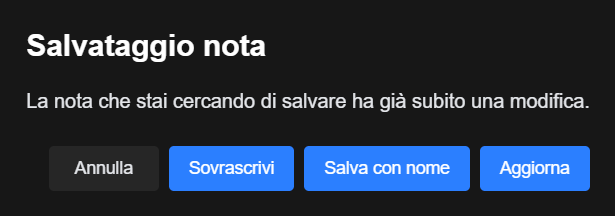
\includegraphics[width=0.65\textwidth]{resources/manual/editor/modale_conflitto_salva.png}
      \caption{Modale per differenza in salvataggio}
      \label{fig:modale_differenza_salva}
    \end{figure}
  \end{center}

  L'utente può quindi decidere quale azione eseguire per risolvere la differenza tra le proprie modifiche e quelle presenti in archivio. Le azioni possibili sono:
    \begin{itemize}
    \item \fcolorbox{black}{cyan!30}{Sovrascrivi} ignora le modifiche esterne ed esegue il salvataggio in archivio con la versione dell'utente
    \item \fcolorbox{black}{cyan!30}{Salva con nome} salva con un nome differente la nota con le modifiche dell'utente (vedi sezione \ref{subsubsec:salva_con_nome})
    \item \fcolorbox{black}{cyan!30}{Aggiorna} ignora le modifiche dell'utente ed aggiorna l'editor con la versione della nota presente nell'archivio
    \item \fcolorbox{black}{gray!30}{Annulla} l'utente declina il salvataggio e procede manualmente alla gestione delle differenze.
    \end{itemize}

  \subsubsection{Esportazione Nota}

  Similmente a come avviene all'interno dell'archivio (vedi sezione \ref{par:esporta_archivio}: esportazione da archivio), è possibile esportare la nota aperta nell'editor cliccando sul bottone \fcolorbox{black}{blue!30}{Esporta} (elemento \#10 nella \autoref{fig:editor_note}). I formati disponibili sono: \texttt{PDF}, \texttt{MD} e \texttt{HTML}.

  \begin{center}
    \begin{figure}[H]
      \centering
      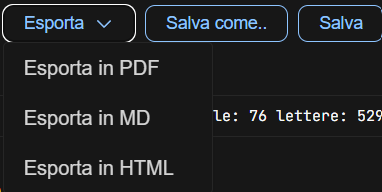
\includegraphics[width=0.45\textwidth]{resources/manual/editor/menu_esporta_editor.png}
      \caption{Menu esportazione nota nell'editor}
      \label{fig:menu_esporta_editor}
    \end{figure}
  \end{center}

  \subsubsection{Salvataggio con Nome}\label{subsubsec:salva_con_nome}

  Similmente a come avviene all'interno dell'archivio (vedi sezione \ref{par:clona_archivio}: clonazione da archivio), è possibile salvare la nota aperta nell'editor con un nome differente cliccando sul bottone \fcolorbox{black}{blue!30}{Salva come...} (elemento \#11 nella \autoref{fig:editor_note}). Verrà presentata una finestra modale per inserire il nome desiderato:

  \begin{center}
    \begin{figure}[H]
      \centering
      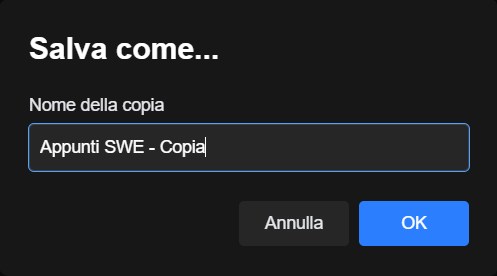
\includegraphics[width=0.45\textwidth]{resources/manual/editor/modale_salva_con_nome.png}
      \caption{Modale per salvataggio con nome}
      \label{fig:salva_come_editor}
    \end{figure}
  \end{center}

Il sistema effettua sempre il controllo di unicità del titolo prima del salvataggio, con i relativi avvisi in base all'esito.
Inoltre in caso di successo viene automaticamente effettuato un reset dell'editor, aggiornato con la copia appena creata.

\newpage

\section{Supporto tecnico}

Per assistenza tecnica relativa all'utilizzo del prodotto software "Second Brain", viene fornito il seguente indirizzo email: 
\begin{center}
    tool8eight@gmail.com
\end{center}
Per un servizio più efficiente, si è pregati di includere nel corpo dell'email una descrizione più completa possibile del problema riscontrato, insieme ad ogni possibile screenshot o dettaglio aggiuntivo che possano risultare utili alla risoluzione di quest'ultimo. \\
Si invita, inoltre, a descrivere eventuali passaggi già tentati per risolvere il problema, in modo che il gruppo possa fornire un'assistenza più mirata.
\end{document}

